\section{Simulation}
We analyze the performance of the maximum likelihood estimators for $\theta$, $\theta_T$, and $\theta_C$ across four parametric copula families: Frank, Clayton, Gumbel, and Gaussian, using lognormal margins for T and C. In the lognormal model, the parameters $\mu$ and $\sigma$ represent the mean and standard deviation of $\log(X)$, respectively, for a lognormal random variable X. Two simulation scenarios are considered, with parameter settings detailed in Table 1. Visualizations of the theoretical density, survival, and hazard functions of Y for each scenario are provided in Figures 1 and 2.

\begin{table}[h]
    \centering
    \caption{Parameter specifications for the simulation scenarios with lognormal margins, with mean parameters \( \mu_T \) and \( \mu_C \) and standard deviation parameters \( \sigma_T \) and \( \sigma_C \) for \( T \) and \( C \), respectively, and dependency measured by Kendall’s \( \tau \)}
    \begin{tabular}{|c|c|c|c|c|c|c|c|c|c|}
        \hline
        Scenario & \( \mu_T \) & \( \sigma_T \) & \( \mu_C \) & \( \sigma_C \) & \( \tau \) & \( \theta_{\text{Frank}} \) & \( \theta_{\text{Clayton}} \) & \( \theta_{\text{Gumbel}} \) & \( \theta_{\text{Gauss}} \) \\
        \hline
        1 & 2.2 & 1.0 & 2.0 & 0.25 & 0.2 & 1.86 & 0.50 & 1.25 & 0.31 \\ 
          &     &     &     &      & 0.5 & 5.74 & 2.00 & 2.00 & 0.71 \\ 
          &     &     &     &      & 0.7 & 11.74 & 4.67 & 3.33 & 0.89 \\ 
        \hline
        2 & 2.5 & 1.0 & 2.0 & 0.50 & 0.2 & 1.86 & 0.50 & 1.25 & 0.31 \\ 
          &     &     &     &      & 0.5 & 5.74 & 2.00 & 2.00 & 0.71 \\ 
          &     &     &     &      & 0.7 & 11.74 & 4.67 & 3.33 & 0.89 \\ 
        \hline
    \end{tabular}
    \label{tab:parameter_specifications}
\end{table}

\begin{figure*}[!h]
	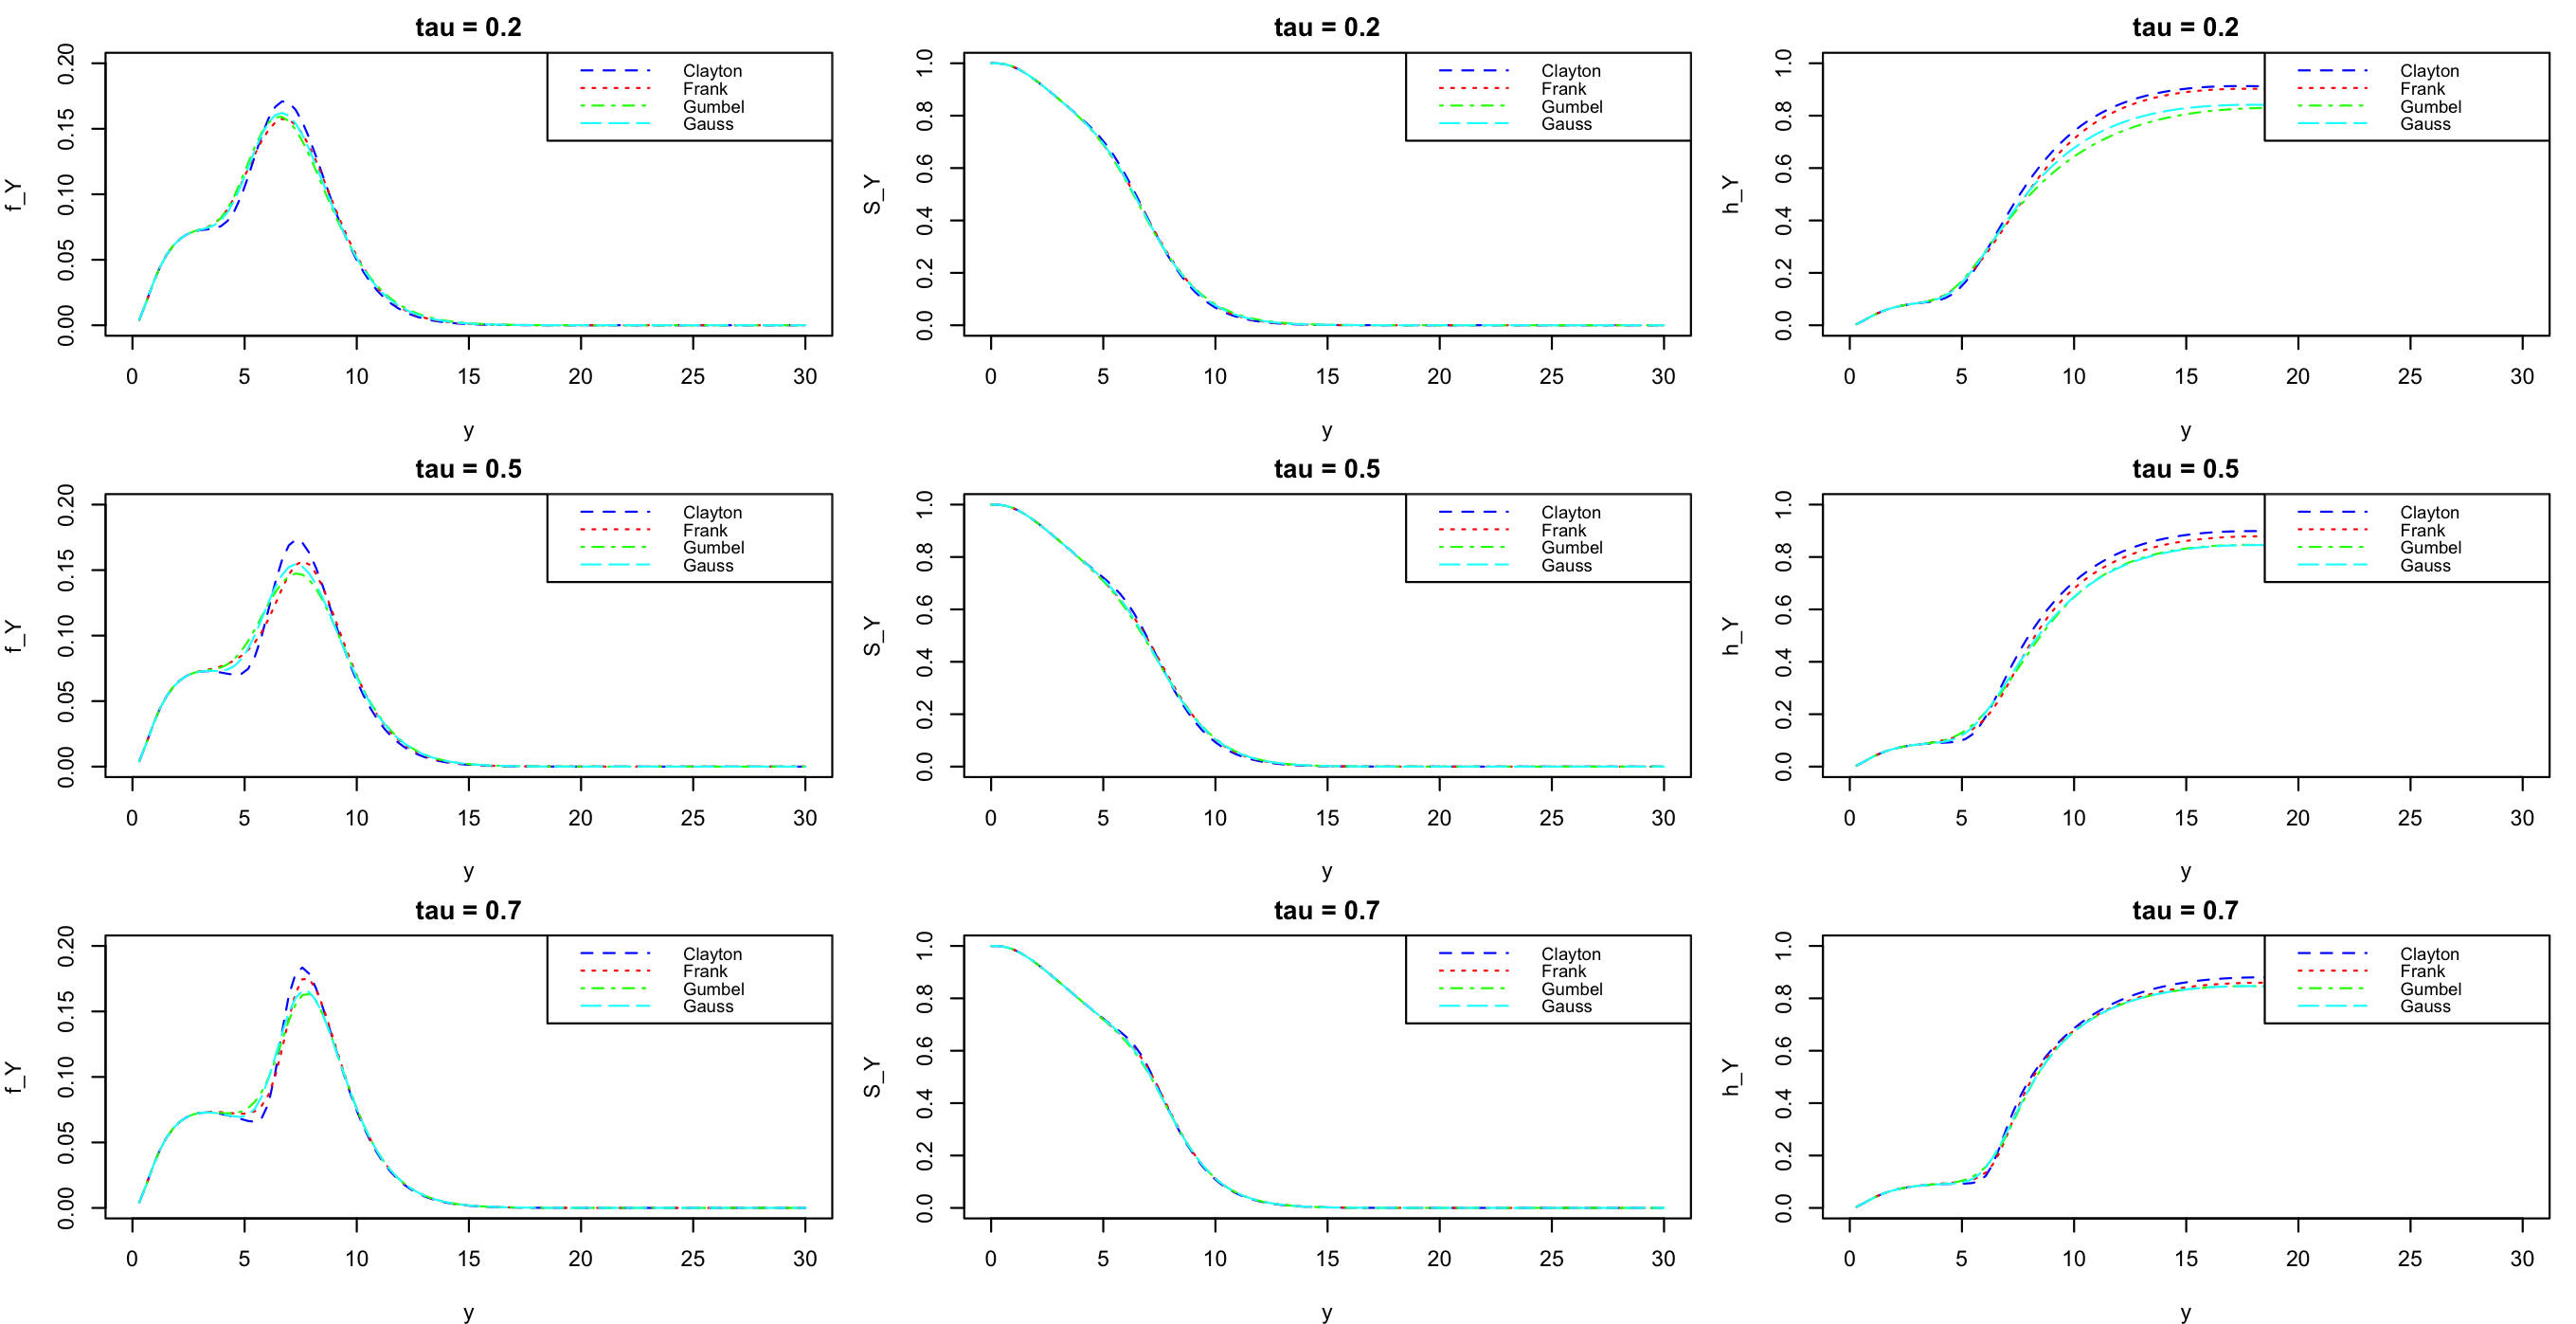
\includegraphics[width=\linewidth]{images/scenario1.png}
	\caption{Theoretical density (left column), survival function (middle column) and hazard (right row) of Y for four copula
families and three τ values under Scenario 1.}
\end{figure*}

\begin{figure*}
	\includegraphics[width=\linewidth]{images/scenario2.png}
	\caption{Theoretical density (left column), survival function (middle column) and hazard (right column) of Y for four copula
families and three τ values under Scenario 2.}
\end{figure*}

In Scenario 1, the marginal density of the observable random variable  is nonstandard, which is anticipated because it results from the sum of two sub-densities. We observe that the strength of dependence between  and  impacts the skewness of $Y$.

We analyze two sample sizes,  and , repeating each simulation setting 100 times. To calculate the asymptotic standard errors, we numerically determine the required Hessian matrix. However, numerical evaluation of the Hessian becomes unstable with extremely large copula parameter values. Therefore, we limit the copula parameter to ensure that the resulting Kendall’s  does not exceed 0.8. This constraint is not overly restrictive, as it corresponds to a correlation of 0.95 in the Gaussian copula. L-BFGS was used as the optimisation algorithm since it is suitable to run on limited amount of computer memory.

For our simulation experiments, we report the average estimate, the empirical standard error of this estimate, the average asymptotic standard error estimates for the parameter estimators, and the empirical root mean squared error based on 100 replications. The results for Scenario 1 are presented in Tables 2, 3, 4, and 5 for the Frank, Clayton, Gumbel, and Gaussian copulas, respectively, demonstrating satisfactory performance of the estimation procedure. As anticipated, the average root mean squared error decreases with an increase in sample size. The marginal parameters are accurately estimated in all cases, and the asymptotic standard error estimates align well with the empirical standard errors.

Moreover, the marginal parameters exhibit nearly perfect unbiasedness even at , leading to an almost exact agreement between the root mean squared error and the empirical standard errors. While 100 Monte Carlo replications may seem limited, the results indicate that this number is adequate.

\begin{table}[h]
    \centering
    \caption{Simulation results for the Frank copula}
    \begin{tabular}{|c|c|c|c|c|c|c|}
        \hline
        & \(\tau\) & \(\mu_T\) & \(\sigma_T\) & \(\mu_C\) & \(\sigma_C\) & Estimated \(\tau\) \\ 
        \hline
        \textbf{n=200} & & & & & & \\
        \hline
        aver.est    & 0.7 & 2.22 & 1.03 & 2.00 & 0.25 & 0.70 \\ 
        sd.aver.est & 0.7 & 0.11 & 0.10 & 0.03 & 0.02 & 0.04 \\ 
        aver.asderr & 0.7 & 0.10 & 0.10 & 0.03 & 0.02 & 0.06 \\ 
        RMSE        & 0.7 & 0.11 & 0.11 & 0.03 & 0.02 & 0.04 \\ 
        \hline
        aver.est    & 0.5 & 2.22 & 1.02 & 2.01 & 0.24 & 0.44 \\ 
        sd.aver.est & 0.5 & 0.13 & 0.12 & 0.05 & 0.02 & 0.18 \\ 
        aver.asderr & 0.5 & 0.11 & 0.10 & 0.04 & 0.02 & 0.14 \\ 
        RMSE        & 0.5 & 0.13 & 0.12 & 0.05 & 0.02 & 0.18 \\ 
        \hline
        aver.est    & 0.2 & 2.26 & 1.00 & 2.00 & 0.25 & 0.22 \\ 
        sd.aver.est & 0.2 & 0.14 & 0.09 & 0.02 & 0.02 & 0.12 \\ 
        aver.asderr & 0.2 & 0.12 & 0.11 & 0.04 & 0.02 & 0.18 \\ 
        RMSE        & 0.2 & 0.15 & 0.08 & 0.02 & 0.02 & 0.12 \\ 
        \hline
        \textbf{n=500} & & & & & & \\
        \hline
        aver.est    & 0.7 & 2.19 & 0.98 & 2.00 & 0.25 & 0.71 \\ 
        sd.aver.est & 0.7 & 0.06 & 0.06 & 0.02 & 0.01 & 0.05 \\ 
        aver.asderr & 0.7 & 0.06 & 0.06 & 0.02 & 0.01 & 0.04 \\ 
        RMSE        & 0.7 & 0.06 & 0.07 & 0.01 & 0.01 & 0.04 \\ 
        \hline
        aver.est    & 0.5 & 2.19 & 0.99 & 2.00 & 0.25 & 0.47 \\ 
        sd.aver.est & 0.5 & 0.08 & 0.07 & 0.03 & 0.02 & 0.08 \\ 
        aver.asderr & 0.5 & 0.07 & 0.06 & 0.02 & 0.01 & 0.08 \\ 
        RMSE        & 0.5 & 0.08 & 0.07 & 0.03 & 0.02 & 0.08 \\ 
        \hline
        aver.est    & 0.2 & 2.18 & 0.96 & 1.99 & 0.25 & 0.25 \\ 
        sd.aver.est & 0.2 & 0.05 & 0.04 & 0.02 & 0.01 & 0.09 \\ 
        aver.asderr & 0.2 & 0.07 & 0.06 & 0.03 & 0.01 & 0.11 \\ 
        RMSE        & 0.2 & 0.06 & 0.06 & 0.03 & 0.01 & 0.10 \\ 
        \hline
    \end{tabular}
    \label{tab:frank_results}
\end{table}

\begin{table}[h]
    \centering
    \caption{Simulation results for the Clayton copula}
    \begin{tabular}{|c|c|c|c|c|c|c|}
        \hline
        & \(\tau\) & \(\mu_T\) & \(\sigma_T\) & \(\mu_C\) & \(\sigma_C\) & Estimated \(\tau\) \\ 
        \hline
        \textbf{n=200} & & & & & & \\
        \hline
        aver.est    & 0.7 & 2.22 & 1.03 & 2.00 & 0.25 & 0.71 \\ 
        sd.aver.est & 0.7 & 0.08 & 0.09 & 0.02 & 0.02 & 0.04 \\ 
        aver.asderr & 0.7 & 0.10 & 0.09 & 0.03 & 0.02 & 0.07 \\ 
        RMSE        & 0.7 & 0.08 & 0.10 & 0.02 & 0.02 & 0.04 \\ 
        \hline
        aver.est    & 0.5 & 2.20 & 1.02 & 2.01 & 0.24 & 0.45 \\ 
        sd.aver.est & 0.5 & 0.10 & 0.08 & 0.05 & 0.03 & 0.18 \\ 
        aver.asderr & 0.5 & 0.10 & 0.09 & 0.04 & 0.03 & 0.17 \\ 
        RMSE        & 0.5 & 0.10 & 0.08 & 0.05 & 0.03 & 0.18 \\ 
        \hline
        aver.est    & 0.2 & 2.16 & 0.96 & 1.99 & 0.26 & 0.25 \\ 
        sd.aver.est & 0.2 & 0.10 & 0.07 & 0.05 & 0.03 & 0.19 \\ 
        aver.asderr & 0.2 & 0.11 & 0.09 & 0.07 & 0.03 & 0.25 \\ 
        RMSE        & 0.2 & 0.10 & 0.08 & 0.05 & 0.03 & 0.20 \\ 
        \hline
        \textbf{n=500} & & & & & & \\
        \hline
        aver.est    & 0.7 & 2.22 & 1.00 & 2.00 & 0.25 & 0.69 \\ 
        sd.aver.est & 0.7 & 0.07 & 0.07 & 0.02 & 0.01 & 0.04 \\ 
        aver.asderr & 0.7 & 0.06 & 0.06 & 0.02 & 0.01 & 0.05 \\ 
        RMSE        & 0.7 & 0.07 & 0.07 & 0.02 & 0.01 & 0.04 \\ 
        \hline
        aver.est    & 0.5 & 2.19 & 1.00 & 2.00 & 0.25 & 0.52 \\ 
        sd.aver.est & 0.5 & 0.07 & 0.07 & 0.02 & 0.02 & 0.07 \\ 
        aver.asderr & 0.5 & 0.06 & 0.06 & 0.02 & 0.02 & 0.09 \\ 
        RMSE        & 0.5 & 0.07 & 0.07 & 0.02 & 0.02 & 0.07 \\ 
        \hline
        aver.est    & 0.2 & 2.18 & 0.98 & 2.01 & 0.25 & 0.19 \\ 
        sd.aver.est & 0.2 & 0.06 & 0.05 & 0.04 & 0.02 & 0.13 \\ 
        aver.asderr & 0.2 & 0.07 & 0.06 & 0.05 & 0.02 & 0.19 \\ 
        RMSE        & 0.2 & 0.06 & 0.06 & 0.04 & 0.02 & 0.12 \\ 
        \hline
    \end{tabular}
    \label{tab:clayton_results}
\end{table}

\begin{table}[h]
    \centering
    \caption{Simulation results for the Gumbel copula}
    \begin{tabular}{|c|c|c|c|c|c|c|}
        \hline
        & \(\tau\) & \(\mu_T\) & \(\sigma_T\) & \(\mu_C\) & \(\sigma_C\) & Estimated \(\tau\) \\ 
        \hline
        \textbf{n=200} & & & & & & \\
        \hline
        aver.est    & 0.2 & 2.21 & 1.00 & 1.99 & 0.25 & 0.24 \\ 
        sd.aver.est & 0.2 & 0.11 & 0.10 & 0.04 & 0.02 & 0.13 \\ 
        aver.asderr & 0.2 & 0.12 & 0.10 & 0.04 & 0.02 & 0.16 \\ 
        RMSE        & 0.2 & 0.10 & 0.10 & 0.04 & 0.02 & 0.13 \\ 
        \hline
        aver.est    & 0.5 & 2.19 & 0.99 & 1.99 & 0.25 & 0.50 \\ 
        sd.aver.est & 0.5 & 0.11 & 0.09 & 0.03 & 0.02 & 0.13 \\ 
        aver.asderr & 0.5 & 0.11 & 0.10 & 0.03 & 0.02 & 0.13 \\ 
        RMSE        & 0.5 & 0.11 & 0.09 & 0.03 & 0.02 & 0.12 \\ 
        \hline
        aver.est    & 0.7 & 2.24 & 1.04 & 2.01 & 0.24 & 0.67 \\ 
        sd.aver.est & 0.7 & 0.11 & 0.07 & 0.02 & 0.02 & 0.05 \\ 
        aver.asderr & 0.7 & 0.11 & 0.10 & 0.03 & 0.02 & 0.08 \\ 
        RMSE        & 0.7 & 0.12 & 0.08 & 0.03 & 0.02 & 0.06 \\ 
        \hline
        \textbf{n=500} & & & & & & \\
        \hline
        aver.est    & 0.2 & 2.19 & 0.98 & 2.00 & 0.25 & 0.22 \\ 
        sd.aver.est & 0.2 & 0.05 & 0.05 & 0.03 & 0.01 & 0.12 \\ 
        aver.asderr & 0.2 & 0.07 & 0.06 & 0.02 & 0.01 & 0.10 \\ 
        RMSE        & 0.2 & 0.06 & 0.05 & 0.03 & 0.01 & 0.12 \\ 
        \hline
        aver.est    & 0.5 & 2.19 & 1.00 & 2.00 & 0.25 & 0.48 \\ 
        sd.aver.est & 0.5 & 0.09 & 0.07 & 0.03 & 0.01 & 0.09 \\ 
        aver.asderr & 0.5 & 0.07 & 0.06 & 0.02 & 0.01 & 0.09 \\ 
        RMSE        & 0.5 & 0.08 & 0.07 & 0.03 & 0.01 & 0.09 \\ 
        \hline
        aver.est    & 0.7 & 2.18 & 0.99 & 2.00 & 0.25 & 0.70 \\ 
        sd.aver.est & 0.7 & 0.07 & 0.05 & 0.02 & 0.01 & 0.04 \\ 
        aver.asderr & 0.7 & 0.06 & 0.06 & 0.02 & 0.02 & 0.05 \\ 
        RMSE        & 0.7 & 0.07 & 0.05 & 0.02 & 0.01 & 0.04 \\ 
        \hline
    \end{tabular}
    \label{tab:gumbel_results}
\end{table}

\begin{table}[h]
    \centering
    \caption{Simulation results for the Gauss copula}
    \begin{tabular}{|c|c|c|c|c|c|c|}
        \hline
        & \(\tau\) & \(\mu_T\) & \(\sigma_T\) & \(\mu_C\) & \(\sigma_C\) & Estimated \(\tau\) \\ 
        \hline
        \textbf{n=500} & & & & & & \\
        \hline
        aver.est    & 0.7 & 2.19 & 1.00 & 2.00 & 0.25 & 0.71 \\ 
        sd.aver.est & 0.7 & 0.05 & 0.07 & 0.02 & 0.01 & 0.04 \\ 
        aver.asderr & 0.7 & 0.06 & 0.06 & 0.02 & 0.01 & 0.04 \\ 
        RMSE        & 0.7 & 0.05 & 0.07 & 0.02 & 0.01 & 0.04 \\ 
        \hline
        aver.est    & 0.5 & 2.20 & 1.00 & 2.00 & 0.25 & 0.48 \\ 
        sd.aver.est & 0.5 & 0.07 & 0.05 & 0.02 & 0.01 & 0.08 \\ 
        aver.asderr & 0.5 & 0.07 & 0.06 & 0.02 & 0.02 & 0.09 \\ 
        RMSE        & 0.5 & 0.07 & 0.05 & 0.02 & 0.01 & 0.08 \\ 
        \hline
        aver.est    & 0.2 & 2.18 & 0.99 & 1.99 & 0.25 & 0.23 \\ 
        sd.aver.est & 0.2 & 0.05 & 0.05 & 0.03 & 0.02 & 0.13 \\ 
        aver.asderr & 0.2 & 0.07 & 0.06 & 0.03 & 0.01 & 0.13 \\ 
        RMSE        & 0.2 & 0.05 & 0.05 & 0.03 & 0.02 & 0.13 \\ 
        \hline
        \textbf{n=200} & & & & & & \\
        \hline
        aver.est    & 0.7 & 2.22 & 1.00 & 2.00 & 0.24 & 0.68 \\ 
        sd.aver.est & 0.7 & 0.09 & 0.08 & 0.02 & 0.02 & 0.08 \\ 
        aver.asderr & 0.7 & 0.11 & 0.09 & 0.03 & 0.02 & 0.08 \\ 
        RMSE        & 0.7 & 0.09 & 0.08 & 0.02 & 0.02 & 0.08 \\ 
        \hline
        aver.est    & 0.5 & 2.23 & 1.03 & 2.00 & 0.25 & 0.46 \\ 
        sd.aver.est & 0.5 & 0.11 & 0.09 & 0.03 & 0.02 & 0.14 \\ 
        aver.asderr & 0.5 & 0.11 & 0.10 & 0.04 & 0.02 & 0.15 \\ 
        RMSE        & 0.5 & 0.11 & 0.09 & 0.03 & 0.02 & 0.14 \\ 
        \hline
        aver.est    & 0.2 & 2.19 & 1.00 & 1.99 & 0.25 & 0.21 \\ 
        sd.aver.est & 0.2 & 0.10 & 0.11 & 0.04 & 0.02 & 0.16 \\ 
        aver.asderr & 0.2 & 0.12 & 0.10 & 0.05 & 0.02 & 0.20 \\ 
        RMSE        & 0.2 & 0.09 & 0.11 & 0.04 & 0.02 & 0.16 \\ 
        \hline
    \end{tabular}
    \label{tab:gauss_results}
\end{table}